\hypertarget{rechnen-in-endlichen-kuxf6rpern}{%
\section{Rechnen in endlichen Körpern}\label{rechnen-in-endlichen-kuxf6rpern}}

\hypertarget{group}{%
\subsection{Group}\label{group}}

Die sogenannte algebraische Gruppe.\\
Damit wir eine Gruppe \textbf{definieren} können: 
\begin{itemize}
    \item Wir brauchen eine Menge von Elementen.
    \item Wir brauchen eine Operation, die jeweils zwei Elemente der Menge verknüpft und ein Resultat liefert.
\end{itemize}

Eine Gruppe hat folgende \textbf{Eigenschaften}: 
\begin{itemize}
    \item Sie ist geschlossen: Wir haben eine Menge und solange wir die Operation anwenden, verlassen wir die Menge nie.
    \item Assoziation: Es spielt keine Rolle, in welcher Reihenfolge ich die Operationen anwende.
    \item Einheitselement: In der Menge muss es ein Element geben, dass ich mit irgendeinem Element verknüpfen kann, ohne dass etwas passiert.
    \item Inverses Element: Zu jedem Element der Menge muss es ein Element geben, dass die Operation rückgängig machen kann.
\end{itemize}

\begin{figure}[H]
\centering
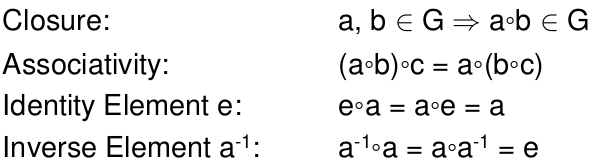
\includegraphics[width=0.5\textwidth]{figures/algebraischeGruppe.png}
\caption{Definitionen Gruppe}
\end{figure}

\hypertarget{abelsche-gruppen-abelian-group}{%
\subsubsection{Abelsche Gruppen (Abelian
Group)}\label{abelsche-gruppen-abelian-group}}

Zusätzlich zu den anderen Regeln gilt noch die kommutative Regel: a verknüpft mit b ergibt dasselbe wie b verknüpft mit a.

\begin{tcolorbox}[colback=red!5!white,colframe=red!75!black]
    Die Menge aller ganzen Zahlen ist z.B. eine abelsche Gruppe.
\end{tcolorbox}

\hypertarget{kuxf6rper-in-englisch-field}{%
\subsection{Körper (in englisch
Field)}\label{kuxf6rper-in-englisch-field}}

Um einen Körper zu \textbf{definieren}, brauchen wir
\begin{itemize}
    \item Eine Menge
    \item Zwei verschiedene Operationen (normalerweise Addition und Multiplikation genannt, aber hat nicht unbedingt etwas mit mathematischer Funktion zu tun.)
\end{itemize}

Ein Körper hat folgende \textbf{Eigenschaften}:
\begin{itemize}
    \item Die Menge F mit der Operation Addition muss eine Abelsche Gruppe sein.
    \item Die Menge F (ohne 0!) mit der Operation Multiplikation muss auch eine Abelsche Gruppe sein.
    \item Die einzige Bedingung, die beide Operationen miteinander verknüpfen, ist das Distributive-Gesetz.
\end{itemize}

\begin{figure}[H]
\centering
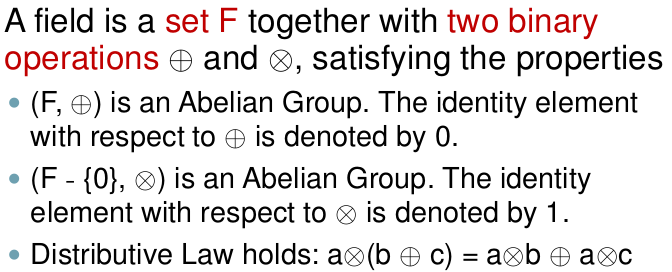
\includegraphics[width=0.5\textwidth]{figures/field.png}
\caption{Definitionen eines Körpers}
\end{figure}

Eigentlich eine Menge, nach
der wir nach gewohnten Regeln addieren und subtrahieren können und auch
multiplizieren und dividieren können, mit einziger Ausnahmen die 0.

\hypertarget{beispiele}{%
\subsubsection{Beispiele}\label{beispiel}}

Die Menge aller ganzen Zahlen: 
\begin{itemize}
    \item Die erste Bedingung mit der Addition ist erfüllt
    \item Die zweite Bedingung ist nicht erfüllt, da eine Multiplikation mit 3 nicht rückgängig gemacht werden kann.
\end{itemize}
\textbf{-> Kein Körper!}

Die Menge aller Bruchzahlen:
\begin{itemize}
    \item Beide Bedingungen werden erfüllt.
\end{itemize}
\textbf{-> Diese Menge bildet einen Körper.}

\hypertarget{allgemeine-eigenschaften-von-kuxf6rpern}{%
\subsubsection{Allgemeine Eigenschaften von
Körpern}\label{allgemeine-eigenschaften-von-kuxf6rpern}}

\begin{itemize}
\tightlist
\item
  Wenn a und b nicht null sind, dann ist auch das Produkt von a und b  nicht null.
\item
  Wenn das Produkt 0 ist, dann muss mindestens einer der beiden Faktoren 0 sein.
\item
  Wenn a nicht 0 ist und es gilt die Beziehung a*b ist a*c, dann ist b =
  c.
\end{itemize}


\begin{figure}[H]
\centering
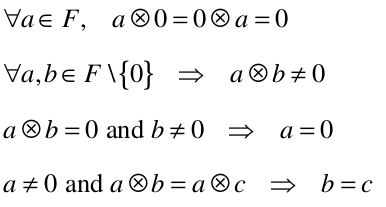
\includegraphics[width=0.5\textwidth]{figures/propertiesOfFields.png}
\caption{Eigenschaften eines Körpers}
\end{figure}

\hypertarget{endliche-kuxf6rper-nennt-man-manchmal-auch-gallua-kuxf6rper-gf}{%
\subsection{Endliche Körper (Nennt man manchmal auch Gallua Körper,
GF)}\label{endliche-kuxf6rper-nennt-man-manchmal-auch-gallua-kuxf6rper-gf}}

\begin{itemize}
\tightlist
\item
  GF(q) ist ein Körper mit einer endlichen Anzahl, nämlich q Elementen.
\item
  Wenn ich das Einheitselement der Multiplikation nehme und das ständig
  addiere, dann ergibt das irgendeinmal 0. Die Kleinste Addition die ich
  dabei brauche, das ist die Charakeristik des Körpers. Dies ist immer
  eine Primzahl.
\item
  Gibt es für jede Zahl q, einen endlichen Körper mit q Elementen?
  -> nein. Die Anzahl Elemente q in einem endlichen Körper
  muss immer Primzahl hoch irgendetwas sein.
\end{itemize}

\begin{figure}[H]
\centering
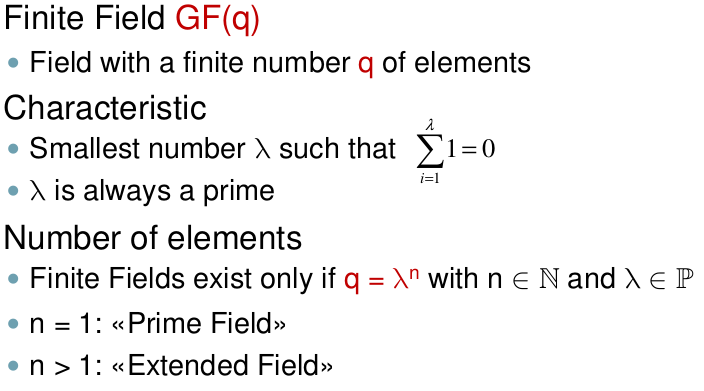
\includegraphics[width=0.5\textwidth]{figures/finiteFields.png}
\caption{Definition endliche Körper}
\end{figure}

\textbf{Es gibt nur zwei Arten von endlichen Körpern.} 
\begin{itemize}
    \item Die Anzahl Elemente ist genau eine Primzahl (n=1 in $GF(q^n)$)
    \item Die Anzahl Elemente ist das Vielfache einer Primzahl $GF(q^{n*k})$
\end{itemize}.

\hypertarget{restklassenkuxf6rper-prime-fields}{%
\subsection{Restklassenkörper (Prime
Fields)}\label{restklassenkuxf6rper-prime-fields}}

\textbf{Endlicher Körper mit Modulo} 
\begin{itemize}
    \item Die Anzahl Elemente ist eine Primzahl
    \item Üblicherweise werden die Elemente des Restklassenkörpers mit den Zahlen 0 bis p-1 dargestellt.
    \item Für die Addition oder die Multiplikation muss der Modulo verwendet werden.
    \item Da alle Elemente von GF(p) teilerfremd zu p sind, gibt es für alle Elemente ein Inverses.
\end{itemize}

\begin{figure}[H]
\centering
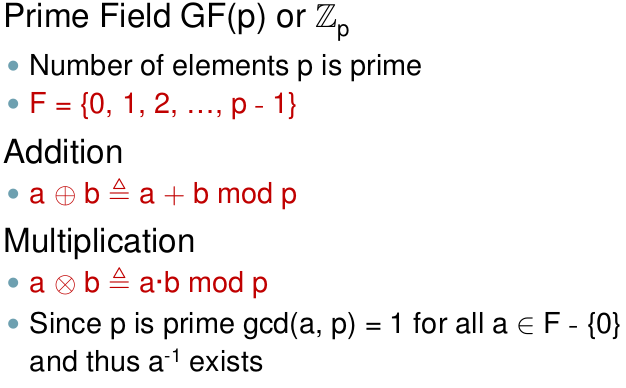
\includegraphics[width=0.5\textwidth]{figures/primeFields.png}
\caption{Definition Prime Field}
\end{figure}

\begin{figure}[H]
\centering
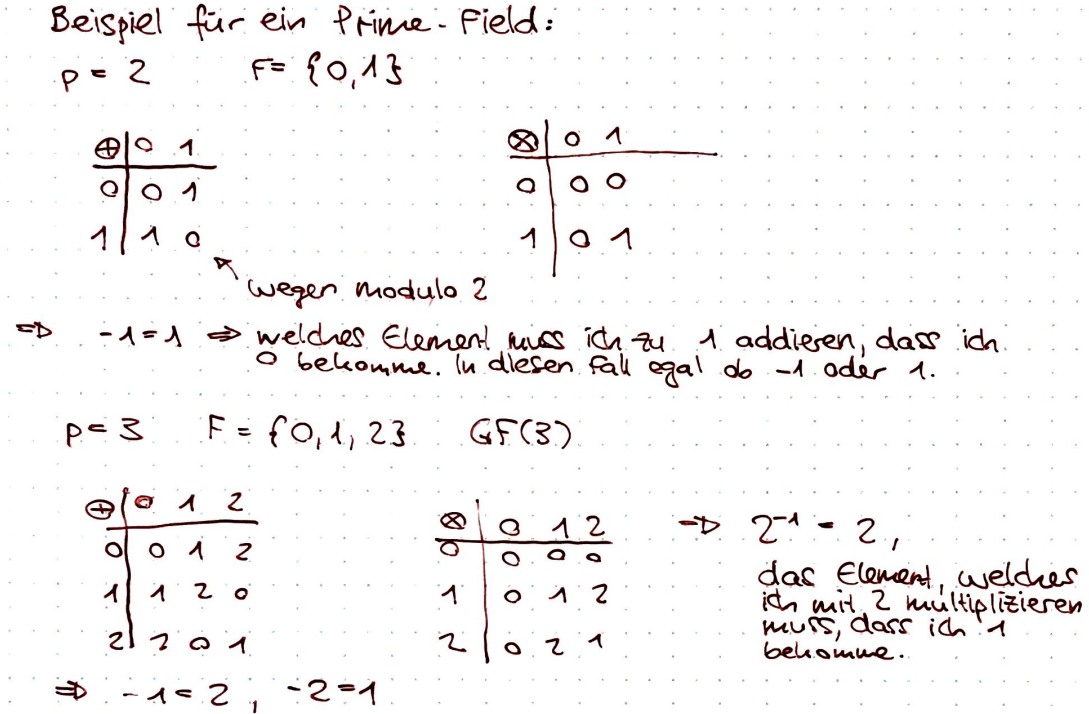
\includegraphics[width=1\textwidth]{figures/notesPrimeField.png}
\caption{Notes Prime Field}
\end{figure}

\hypertarget{polynome}{%
\subsection{Polynome}\label{polynome}}

\begin{itemize}
\tightlist
\item
  Rechenvorschrift, wie man ein Resultat p errechnet mit x.
\item
  Die höchste Potenz, die vorkommt, das ist der Grad des Polynoms.
\item
  Der dazugehörigen Koeffizient der höchsten Potenz, ist der
  Leitkoeffizient.
\item
  Die Menge aller Polynome mit Koeffizienten aus dem Körper F schreibt
  man F{[}x{]}.
\end{itemize}

\begin{figure}[H]
\centering
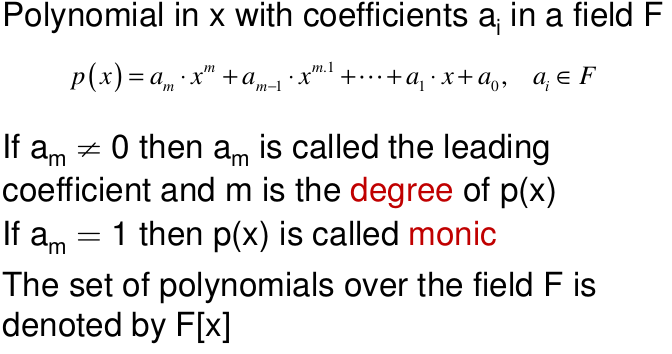
\includegraphics[width=0.5\textwidth]{figures/polynomials.png}
\caption{Definition Polynome}
\end{figure}

\hypertarget{beispiele-polynome}{%
\subsubsection{Beispiele Polynome}\label{beispiel-2}}

\begin{figure}[H]
\centering
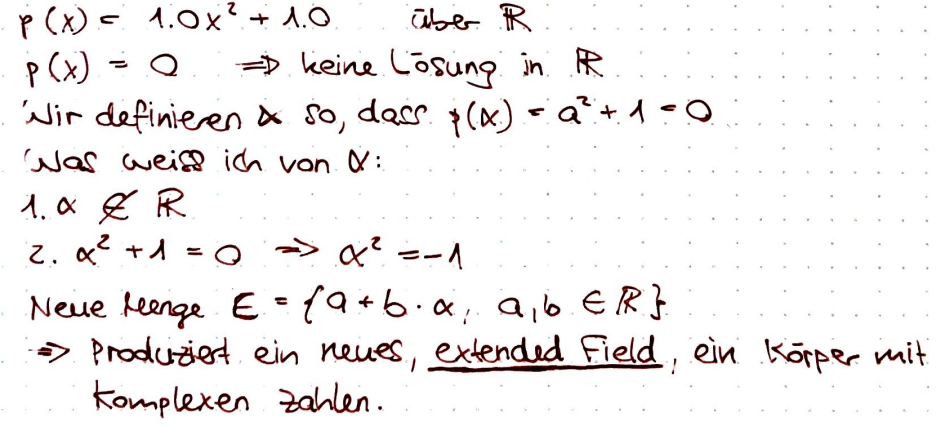
\includegraphics[width=0.8\textwidth]{figures/notesPolynome.png}
\caption{Notes Polynome}
\end{figure}

\hypertarget{nicht-reduzierbare-polynome-irreducible-polynomials}{%
\subsubsection{Nicht reduzierbare Polynome (Irreducible
Polynomials)}\label{nicht-reduzierbare-polynome-irreducible-polynomials}}

\begin{itemize}
\tightlist
\item
  Normalerweise kann ein Polynom reduziert werden. Statt x Quadrat macht man einfach x * x.
\item
  Gewisse Polynome sind nicht reduziertbar, je nach Körper. Diese nennt man irreducible.
\end{itemize}

\hypertarget{erweiterte-kuxf6rper-extended-fields}{%
\subsection{Erweiterte Körper (Extended
Fields)}\label{erweiterte-kuxf6rper-extended-fields}}

\begin{itemize}
\tightlist
\item
  Zum Start wird ein Polynom m(x) mit Grad n \textgreater{} 1 benötigt,
  das nicht reduzierbar ist und vom Körper F stammt.
\item
  Die Elemente vom erweiterten Körper E sind alle Polynome von F{[}x{]},
  welche maximal den Grad n-1 haben.
\end{itemize}

\begin{figure}[H]
\centering
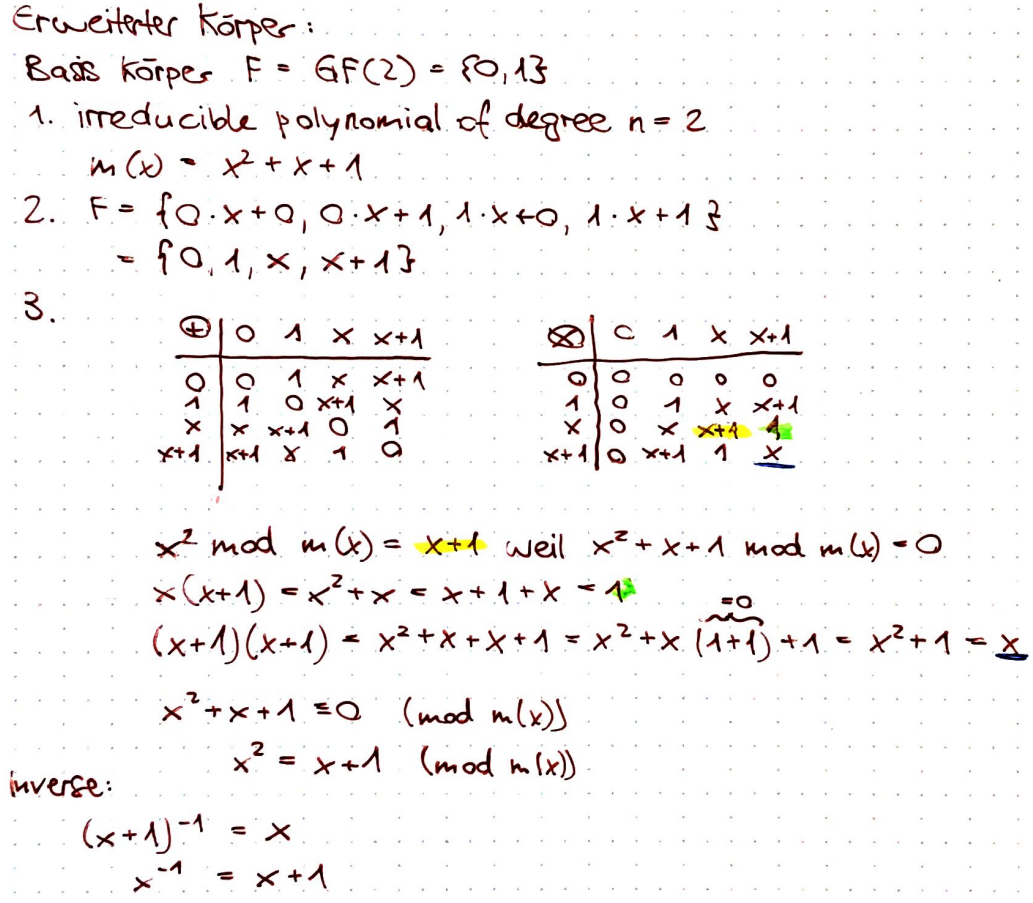
\includegraphics[width=0.8\textwidth]{figures/erweiterterKoerper.png}
\caption{Erweiterter Körper}
\end{figure}

In diesem Beispiel ist x ein primitives oder erzeugendes Element, da
$x^n$ für $n = 0,1,2$ alle Elemente (ausser 0) des erweiterten Körpers
erzeugt.\\
Dies ist nicht immer so, sondern in diesem Fall nur weil unser Polynom
ein unreduzierbares, primitives Polynom ist.

\hypertarget{primitive-polynomial}{%
\subsection{Primitive Polynomial}\label{primitive-polynomial}}

\begin{itemize}
\tightlist
\item
  Ein primitives Polynom muss unreduziertbar sein
\item
  Ein primitives Polynom hat ein primitives Element, welches alle
  Elemente des erweiterten Körpers erzeugen kann.
\item
  Diese primitive Polynome lesen wir oft einfach in einer Tabelle ab.
\end{itemize}

\begin{figure}[H]
\centering
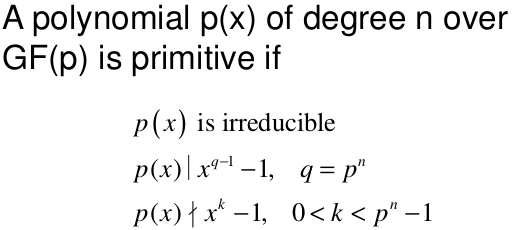
\includegraphics[width=0.3\textwidth]{figures/primitivePolynomial.png}
\caption{Definition primitives Polynom}
\end{figure}

\begin{figure}[H]
\centering
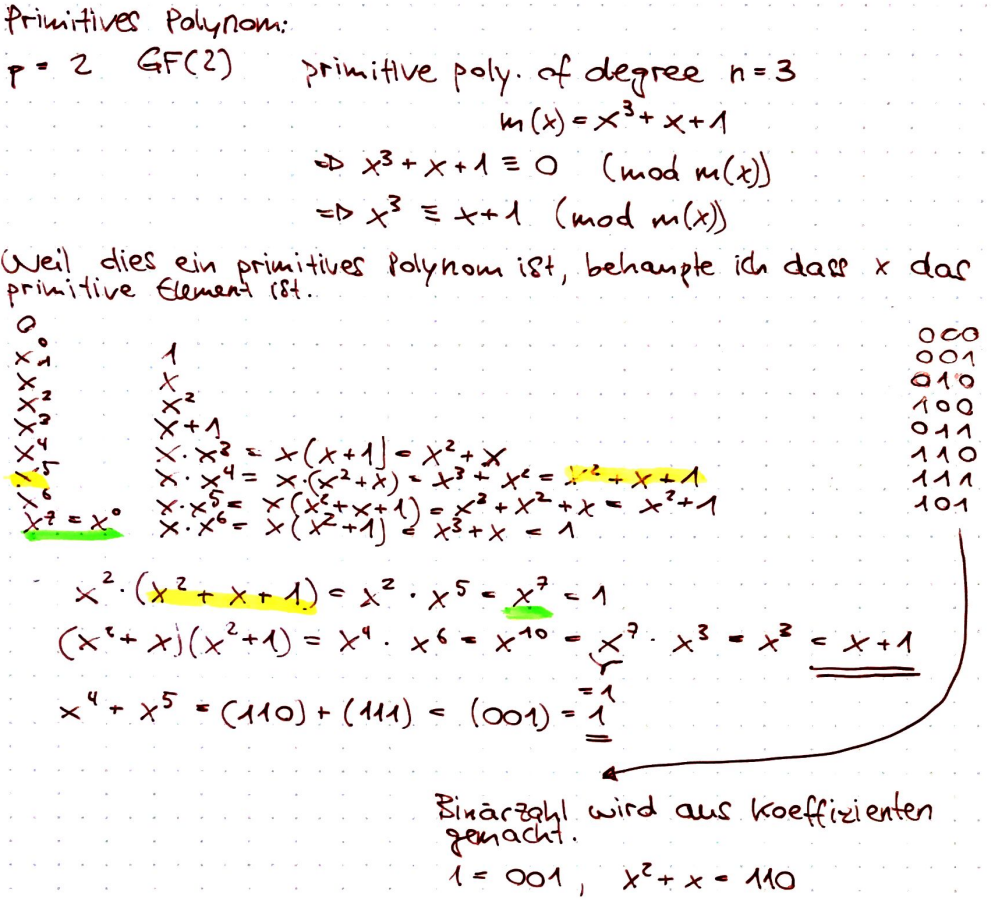
\includegraphics[width=1\textwidth]{figures/primitivesPolynom.png}
\caption{Primitives Polynom}
\end{figure}

\clearpage